\title{Writing Shellcode and Exploiting Stack Overflows on x86 and ARM}
\author{
    Author: Yusef Karim \\
    Instructor: Jacques Béland \\
    Department of Computing \& Information Systems \\
}
\date{\today}

\documentclass[12pt]{article}
\usepackage[utf8]{inputenc}
\usepackage[english]{babel}
\usepackage[a4paper,margin=1in,footskip=0.25in]{geometry}
\usepackage[colorlinks=true]{hyperref}
\usepackage{graphicx}
\usepackage{float}

\begin{document}
\maketitle
\tableofcontents

\section{Purpose}
We will be finishing the last parts of chapter 2 and starting chapter 3 in this lab. These chapters focus on writing and testing shellcode, which is injectable machine instructions we can insert into memory to be executed. We will be expanding upon the information gained from these chapters by attempting to write shellcode and carry out exploits on an ARM architecture. All x86 progress shown below will be within the Ubuntu 16.04 VM, while any ARM progress will be run on our Raspberry Pi.

\section{Before we begin}
Before learning how to write and test shellcode, we should do a quick review of assembly language for both x86 and ARM. One thing to note is that the course text uses the \textit{nasm} assembler to create object files, but below the GNU \textit{as} assembler will be used instead. We will be creating a simple program for both architectures that prints a message then exits. These programs are included in their own respective directories and have been fully commented, named \textit{hello.s}. Images of the code and how to create an executable using an assembler and linker are shown below:

\begin{figure}[H]
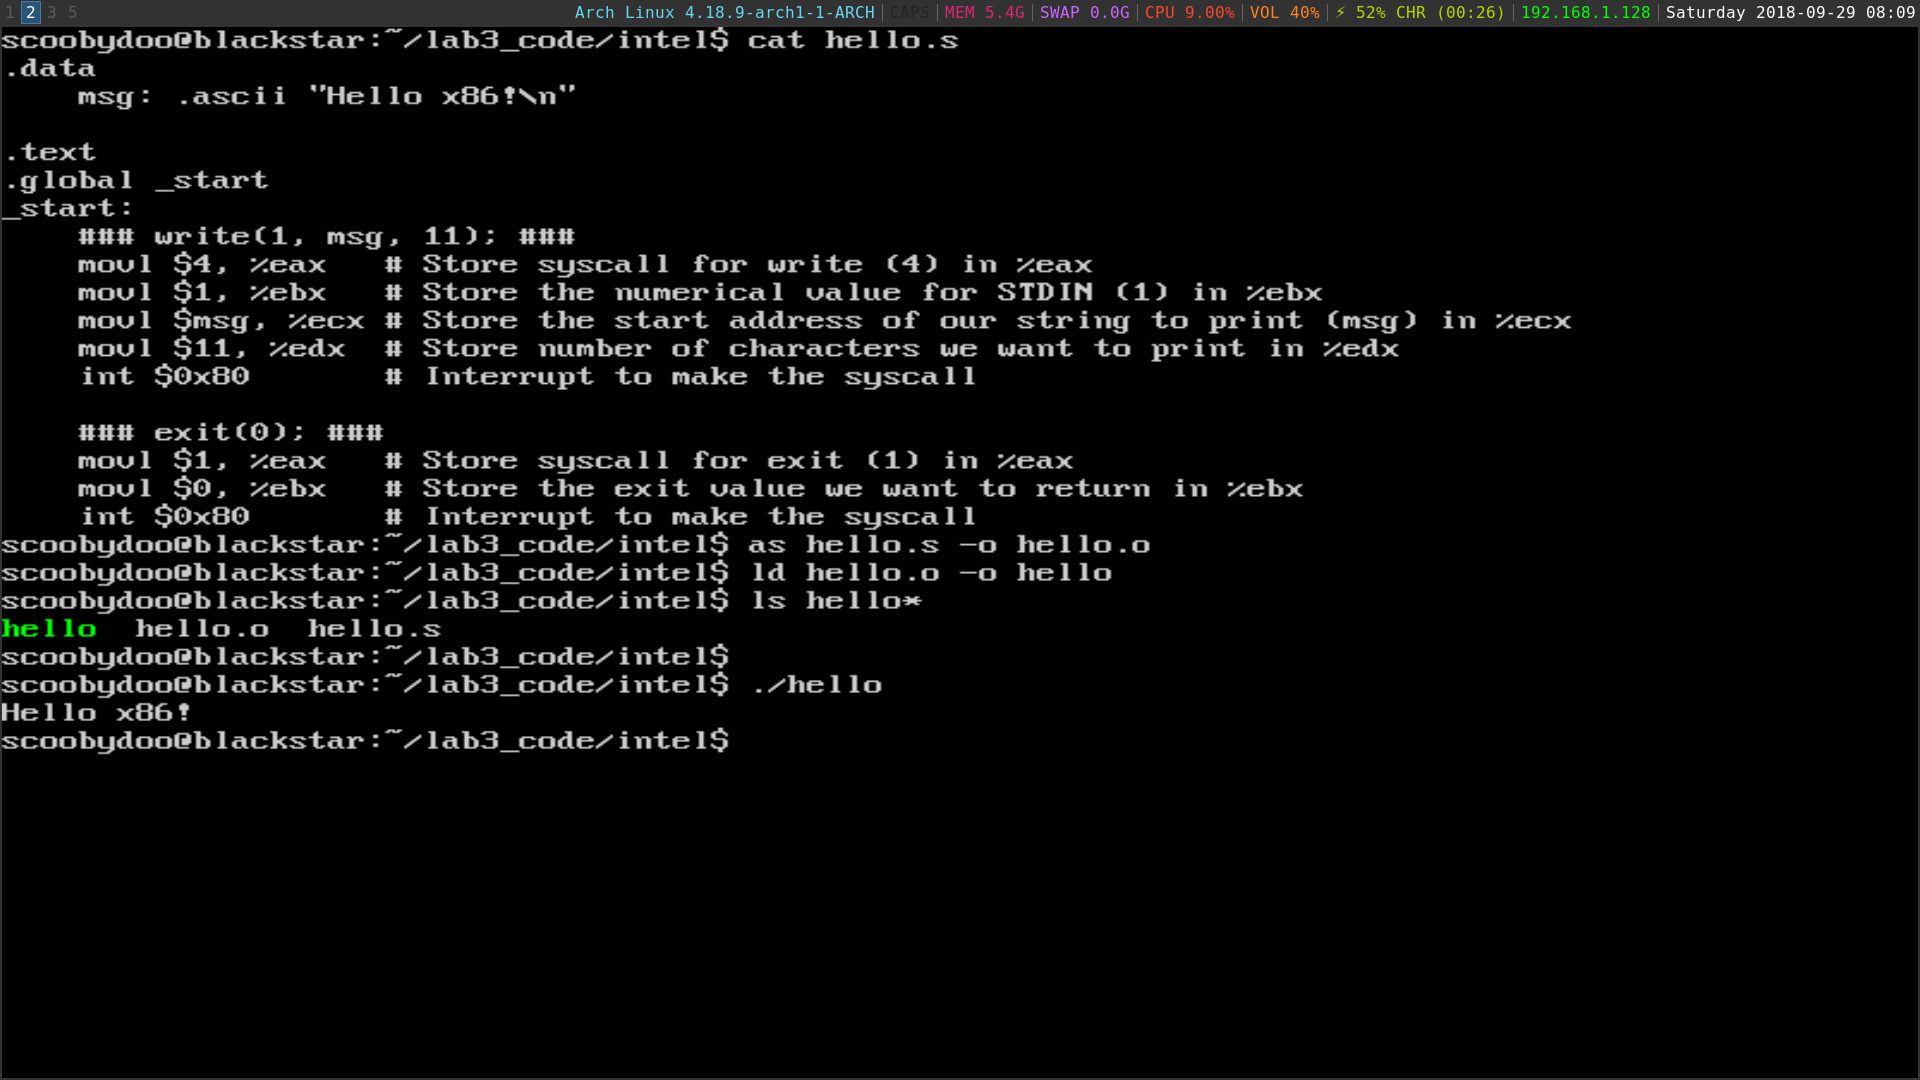
\includegraphics[width=15cm, height=8cm]{hello_x86.png}
  \caption{Assembling and linking our x86 assembly code}
\end{figure}

\begin{figure}[H]
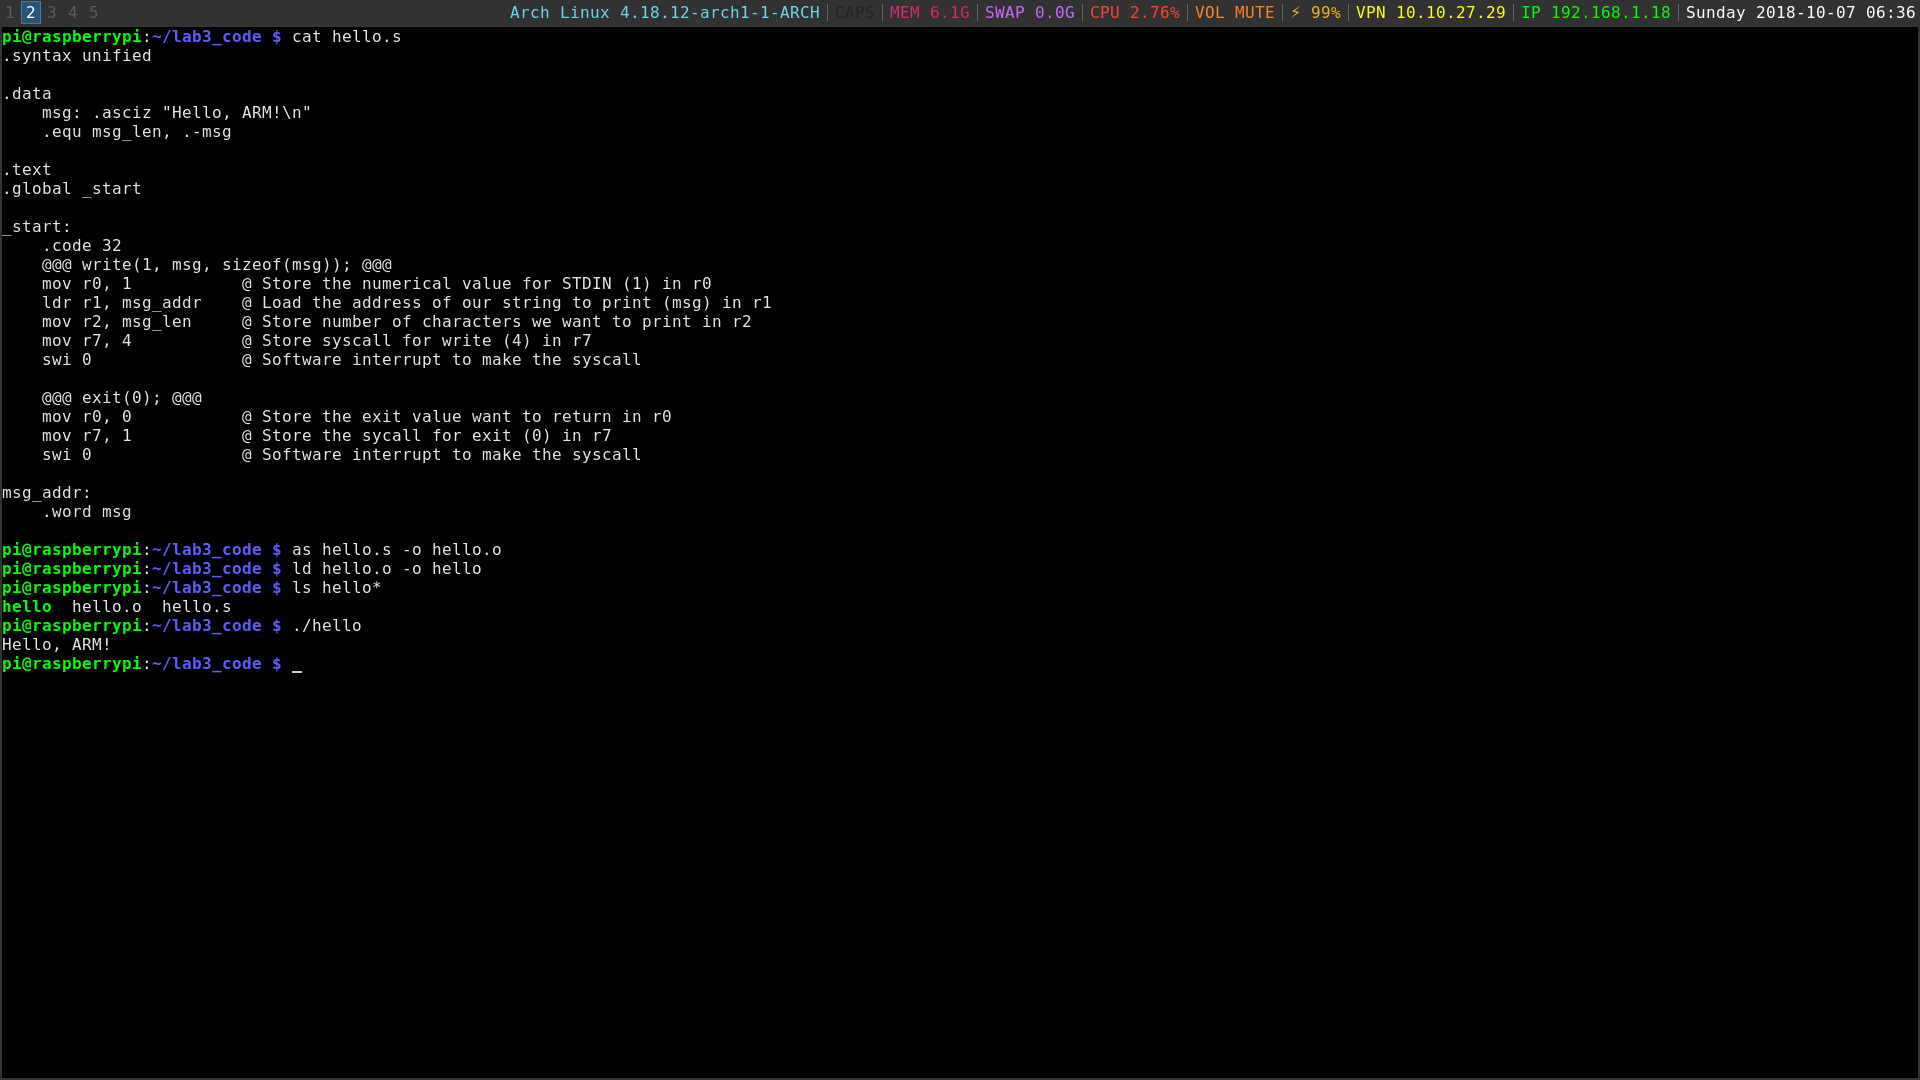
\includegraphics[width=15cm, height=8cm]{hello_ARM.png}
  \caption{Assembling and linking our ARM assembly code}
\end{figure}

\section{How to test your shellcode}
Before learning how to write our own shellcode we need a way to test the shellcode we write. The course text gives a nice little C program to do just this (pages 26-27) but the code did not properly work for me, thus a new version of the \textit{shellcode.c} program has been written and commented to correct this. Another addition is a Python script (shellcode.py) that achieves that same thing with a couple of advantages. The C program \textit{shellcode.c} must be compiled with the options:
\begin{verbatim}
gcc shellcode.c -z execstack -o shellcode
\end{verbatim}
This makes the individual pages of the stack executable, which is required for our shellcode to be executed. The included Python program does away with this. By using the built-in ctypes library the script sets the memory pages as executable using the \textit{mprotect} libc function.
\newline\textbf{NOTE:} This could also be done in C directly, Python is just fun.\newline

The Python script \textit{shellcode.py} is based \textbf{heavily} on a Stack Overflow post [2] but was commented thoroughly using information found in the GNU manuals [3]. In the next chapter, we will learn how to write shellcode, which we can then test using the programs explained above.

\section{Creating your own custom shellcode}
We can now try creating our very own shellcode, much of the theory and process in this section is taken from chapter 3 of the course text. When writing shellcode you must first identify what you want to achieve, then get an idea of what system calls you will need to call, finally you must figure a way to write assembly code that is minimal and flexible. Once this is achieved you can use \textit{gdb} or \textit{objdump} to dump the opcode values (machine instructions) that will make up your shellcode. To demonstrate this process, we will be making shellcode that spawns a \textit{sh} shell on both x86 and ARM.
\subsection{x86 shell}
We will be using the \textit{execve} syscall to help us spawn a shell, then call the \textit{exit} function to terminate the program we are inserting our shellcode into. Looking at the list of Linux syscalls [5] we can see the call to \textit{execve} is 11, and the syscall for \textit{exit} is 1. In section 2 of this lab we learned how to pass arguments then make a syscall, all we need to know is what arguments \textit{execve} takes, which can easily be obtained from the man pages (man execve).\newline

The first thing was to write something that worked, then things such as reducing the size and getting rid of NULL bytes were done, the results of this are shown in the files \textit{bad\_shell.s} and \textit{good\_shell.s} respectively (in the intel directory). One thing to note is when writing these I found the Linux tool \textit{strace} was useful to see what was happening when I made system calls.
\begin{figure}[H]
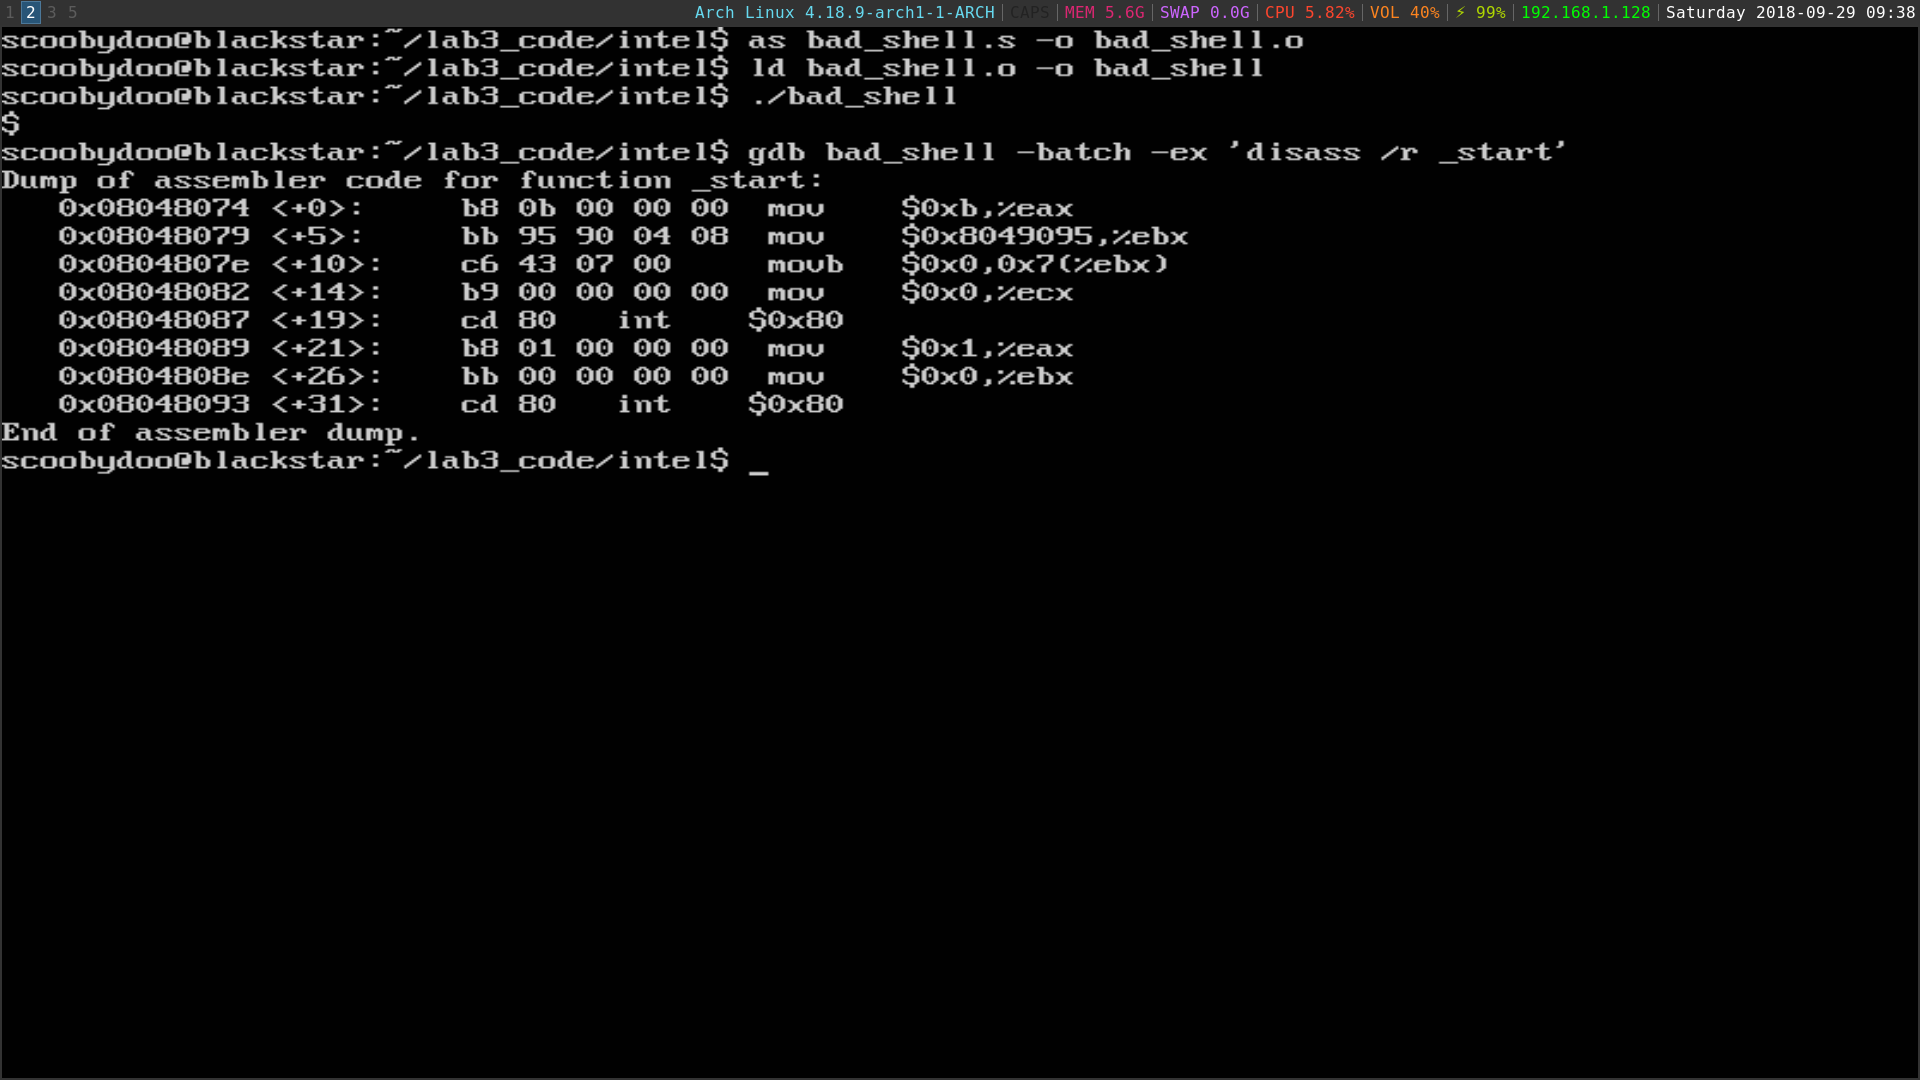
\includegraphics[width=15cm, height=8cm]{bad_shell_x86.png}
  \caption{Creating, running, and disassembling x86 bad\_shell.s}
\end{figure}

From the disassembly of \textit{bad\_shell.s} we can see there is a whopping 14 NULL bytes in our shellcode, they got to go. The results of getting rid of the NULL bytes is shown in the figure below. Please note that the method used was VERY different than the solution in the text book. The method below was fully inspired by the shellcode from exploit-db.com, the execve code [7] and exit code [8] were combined and commented fully in the file \textit{good\_shell.s}, also note a function called \textit{stringToLittleEndianHex} was written in \textit{shellcode.py} to help understand how to get the arguments needed for the execve function into hexadecimal format. This method allowed us to make a much more compact shellcode that also exits cleanly, whilst also making it many times harder for the marker to mark ;).
\begin{figure}[H]
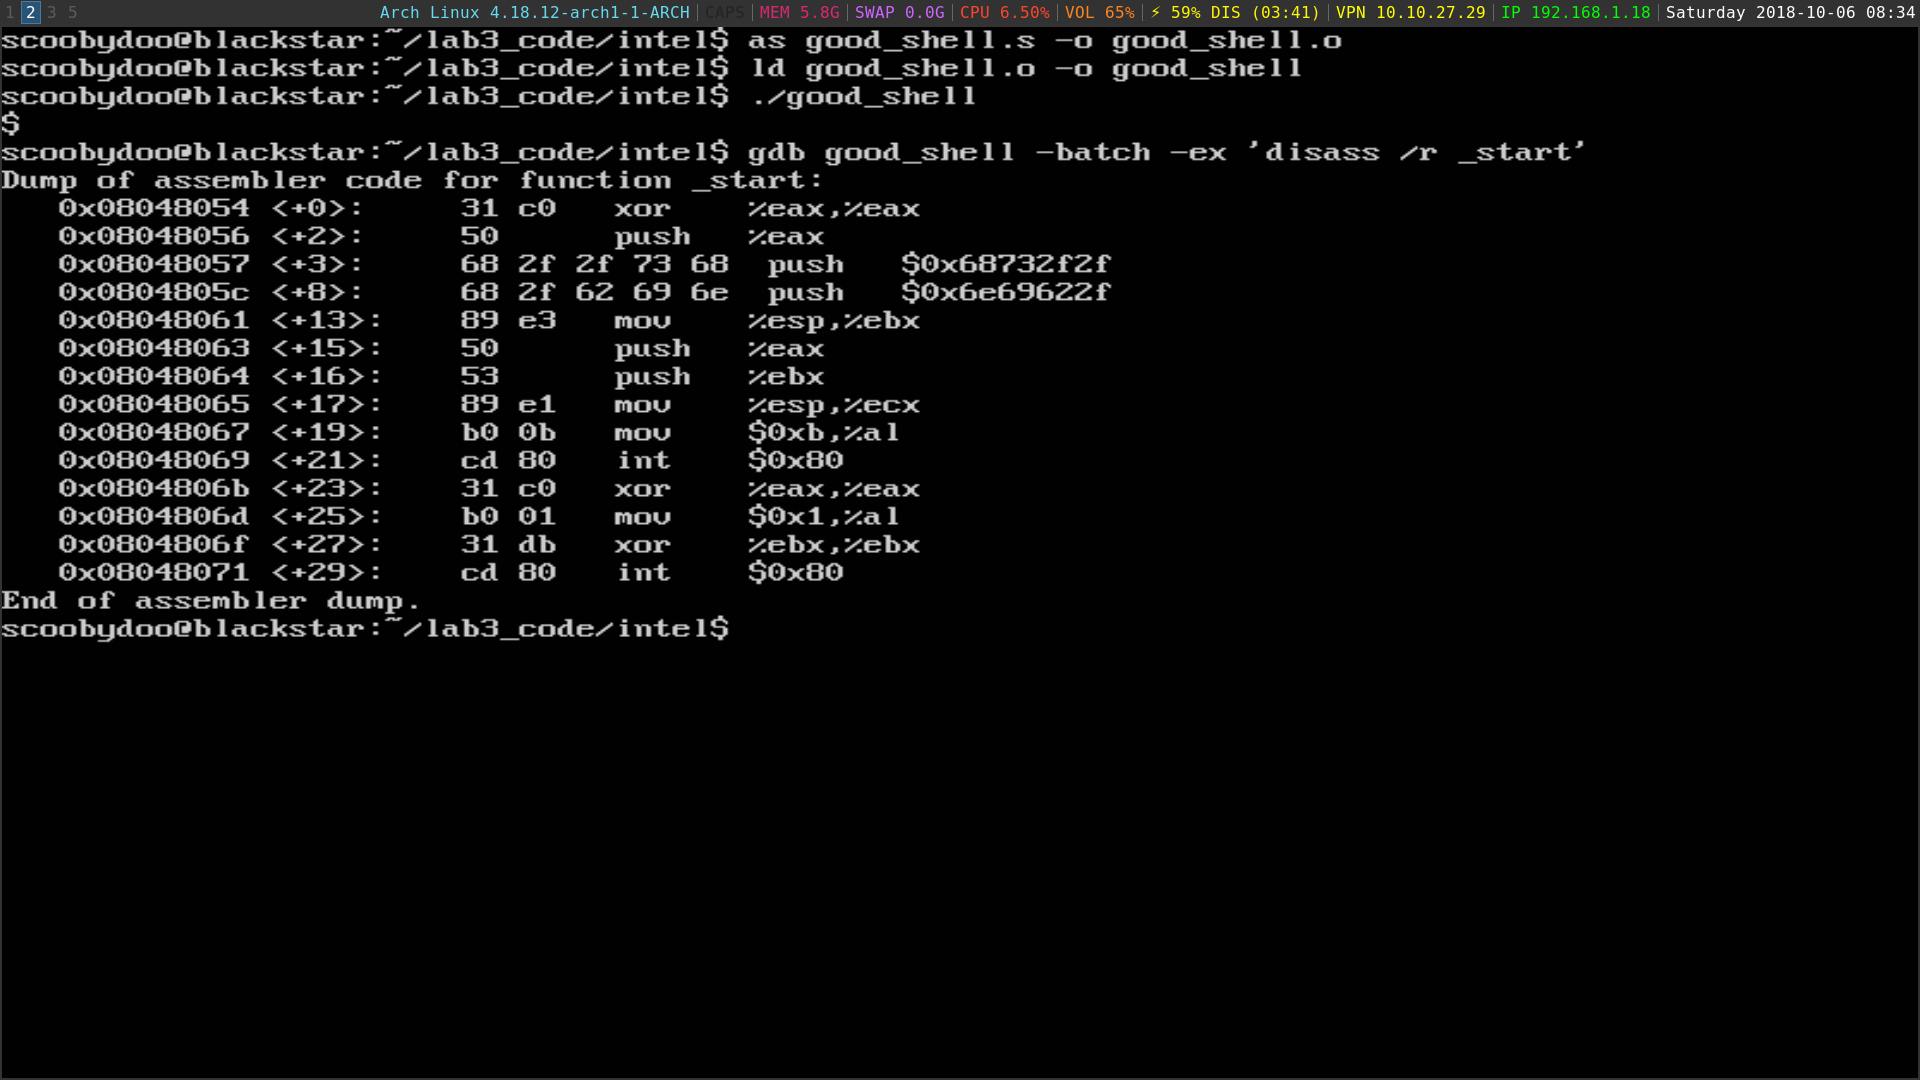
\includegraphics[width=15cm, height=8cm]{good_shell_x86.png}
  \caption{Creating, running, and disassembling x86 good\_shell.s, no NULL bytes woohoo!}
\end{figure}

\subsection{ARM shell}
Similar steps were taken to create the shellcode for the Raspberry Pi (Raspbian), first assembly was written to get a general idea of how to call execve and make system calls using the ARM architecture, shown below:
\begin{figure}[H]
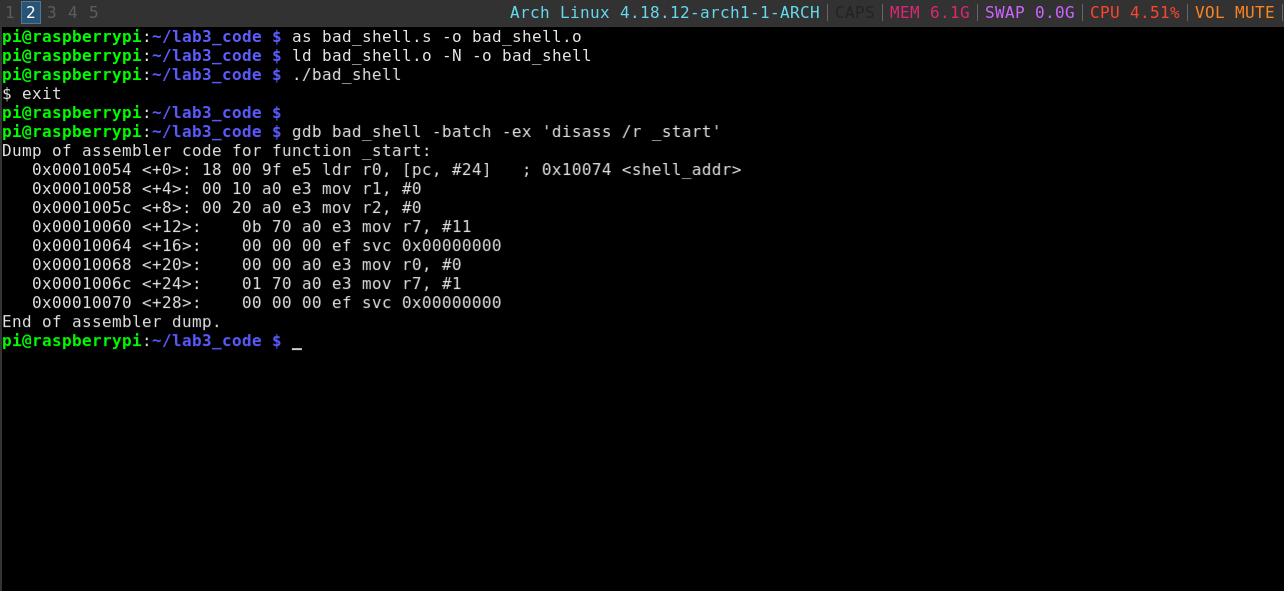
\includegraphics[width=15cm, height=8cm]{bad_shell_arm.png}
  \caption{Creating, running, and disassembling ARM bad\_shell.s}
\end{figure}
This time we have 11 NULL bytes we need to get rid of. Initially, resources from the blog Azeria Labs [9] were used to learn about the steps needed to be taken, then with help from shellcode posted on exploit-db [10] execve shellcode was created and commented in \textit{good\_shell.s} within the arm directory, shown below:
\begin{figure}[H]
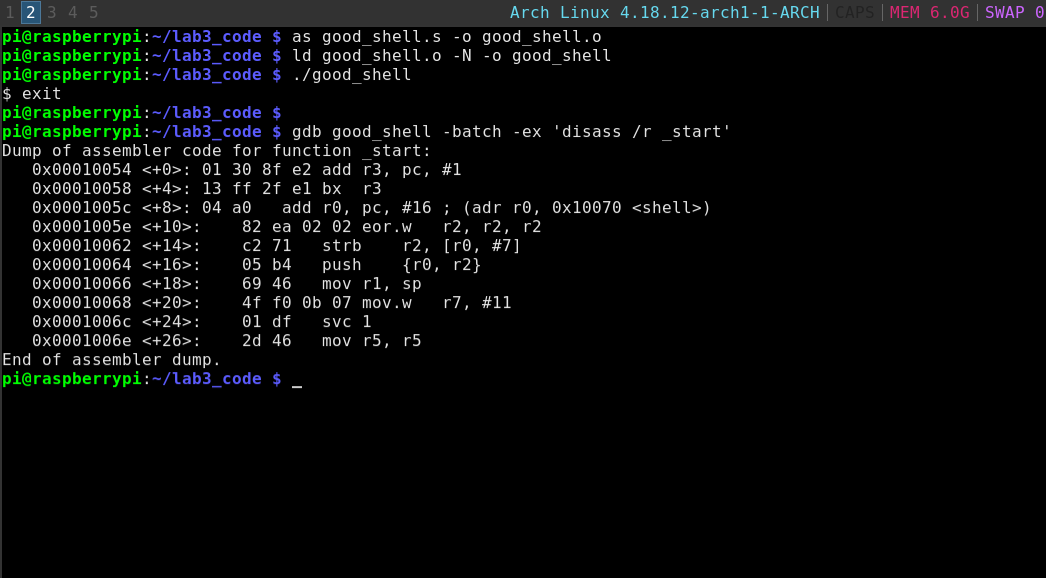
\includegraphics[width=15cm, height=8cm]{good_shell_arm.png}
  \caption{Creating, running, and disassembling ARM good\_shell.s, no NULL bytes yippee!}
\end{figure}
The main things to take note of is the fact that you can use a branch and exchange (BX) instruction in ARM to change the instruction mode. If you use a destination address with the least significant bit (LSB) set to 1 with the \textbf{BX} instruction you will change over to THUMB mode which uses 16 bit instructions instead of 32 bit, this reduces the chance our opcodes will contain NULL bytes. Another thing is the \textbf{ADR} instruction which is a pseudo instruction that uses  program-relative adressing to offset from the current value of the \textit{Program Counter} (PC) register to store the address of our "/bin/sh" string. Finally, in our shellcode we are required to edit the string which exists in the .text segment of our program, this means we must pass the -N argument to our linker which will make the .text section writable.
\begin{verbatim}
ld good_shell.o -N -o good_shell
\end{verbatim}
While writing these assembly snippets, a function called \textit{printShellcode()} was created in \textit{shellcode.py} which will take the assembled and linked exectuable you have made and use the objcopy command to create a binary file, extract the opcodes from that file, and print them nicely out for you.

\subsection{Conclusion}
We have now successfully created shellcode that uses execve to spawn a shell in both x86 and ARM. Using the function \textit{printShellcode()} in \textit{shellcode.py} we can see the results of our effort.
\newline\newline\textbf{x86}
\begin{verbatim}
./shellcode.py
Shellcode for good_shell has length: 31
\x31\xc0\x50\x68\x2f\x2f\x73\x68\x68\x2f\x62\x69\x6e\x89\xe3\x50\x53\x89\xe1\xb0\x0b
\xcd\x80\x31\xc0\xb0\x01\x31\xdb\xcd\x80
\end{verbatim}
\textbf{ARM}
\begin{verbatim}
./shellcode.py
Shellcode for good_shell has length: 36
\x01\x30\x8f\xe2\x13\xff\x2f\xe1\x04\xa0\x82\xea\x02\x02\xc2\x71\x05\xb4\x69\x46\x4f
\xf0\x0b\x07\x01\xdf\x2d\x46\x2f\x62\x69\x6e\x2f\x73\x68\x58
\end{verbatim}

\section{Exploiting victim.c and overflow.c}
Now that we have created our own shellcode we can try to make a vulnerable program execute it. The course text provides a very simple program called \textit{victim.c} that takes an argument from the command line and copies it into a buffer with a fixed size. The error in this program is that it does not restrict the number of characters copied into the buffer. We will take advantage of this in two different ways then discuss the advantages of each method. All the code for this section is in the \textit{exploit} directory. Also note, the \textit{victim.c} program was slightly changed (smaller buffer) so it is easier to show the debugging process.
\subsection{NOP method}

The basics of the NOP method is to have our shellcode stored somewhere (either directly in program memory or in an environment variable) then overflow the buffer in a correct way to have the memory address of our shellcode overwrite the instruction pointer (EIP or PC for ARM). If we overwrite the instruction pointer with the correct memory address the target program will jump to that location and start executing our shellcode. NOP stands for NO Opeartion and it is an assembly instruction that does nothing, since it does nothing the instruction pointer will just move on to the next instruction. If we have many NOP instructions the instruction pointer will just keep going until it hits proper code (our shellcode!), this is why some people call it a NOP sled. The reason to use a NOP sled is because it allows us to get the memory address needed to overwrite the instruction pointer slightly wrong. If we overwrite with an address before our shellcode by mistake the instruction pointer will simply slide down the NOP sled until it gets to our shellcode.\newline

Instead of injecting our shellcode directly into program memory I chose to use the environment variable method, in my opinion this gives us more slack when guessing the memory location. While learning about the ROP method a (over the top) python script was made to help in exploitation, it is called \textit{nop.py}.
\subsubsection{x86}
To start let's compile the victim:
\begin{verbatim}
gcc victim.c -fno-stack-protector -z execstack -mpreferred-stack-boundary=2
-o victim
\end{verbatim}
Next, let's use GDB to see what's going on and how we can overflow the program. The \textit{nop.py} has an optional command (-d) that prints a buffer of repeating letters of specified size, let's use that.\newline

In the figure below you can see we set a breakpoint right after the strcpy function, using the nop.py script to print a string of size 202 we see the program runs fine, no overflow. Next, we run it again this time with a buffer size of 208, this time it crashes saying the address it was trying to return to. If we print the memory around the stack pointer we see that all the addresses have been overwritten by our buffer. In fact, 0x5a5a5a5a is just the four Z characters from our buffer. We now know we need a buffer of at least 208 to overwrite EIP.\newline


\begin{figure}[H]
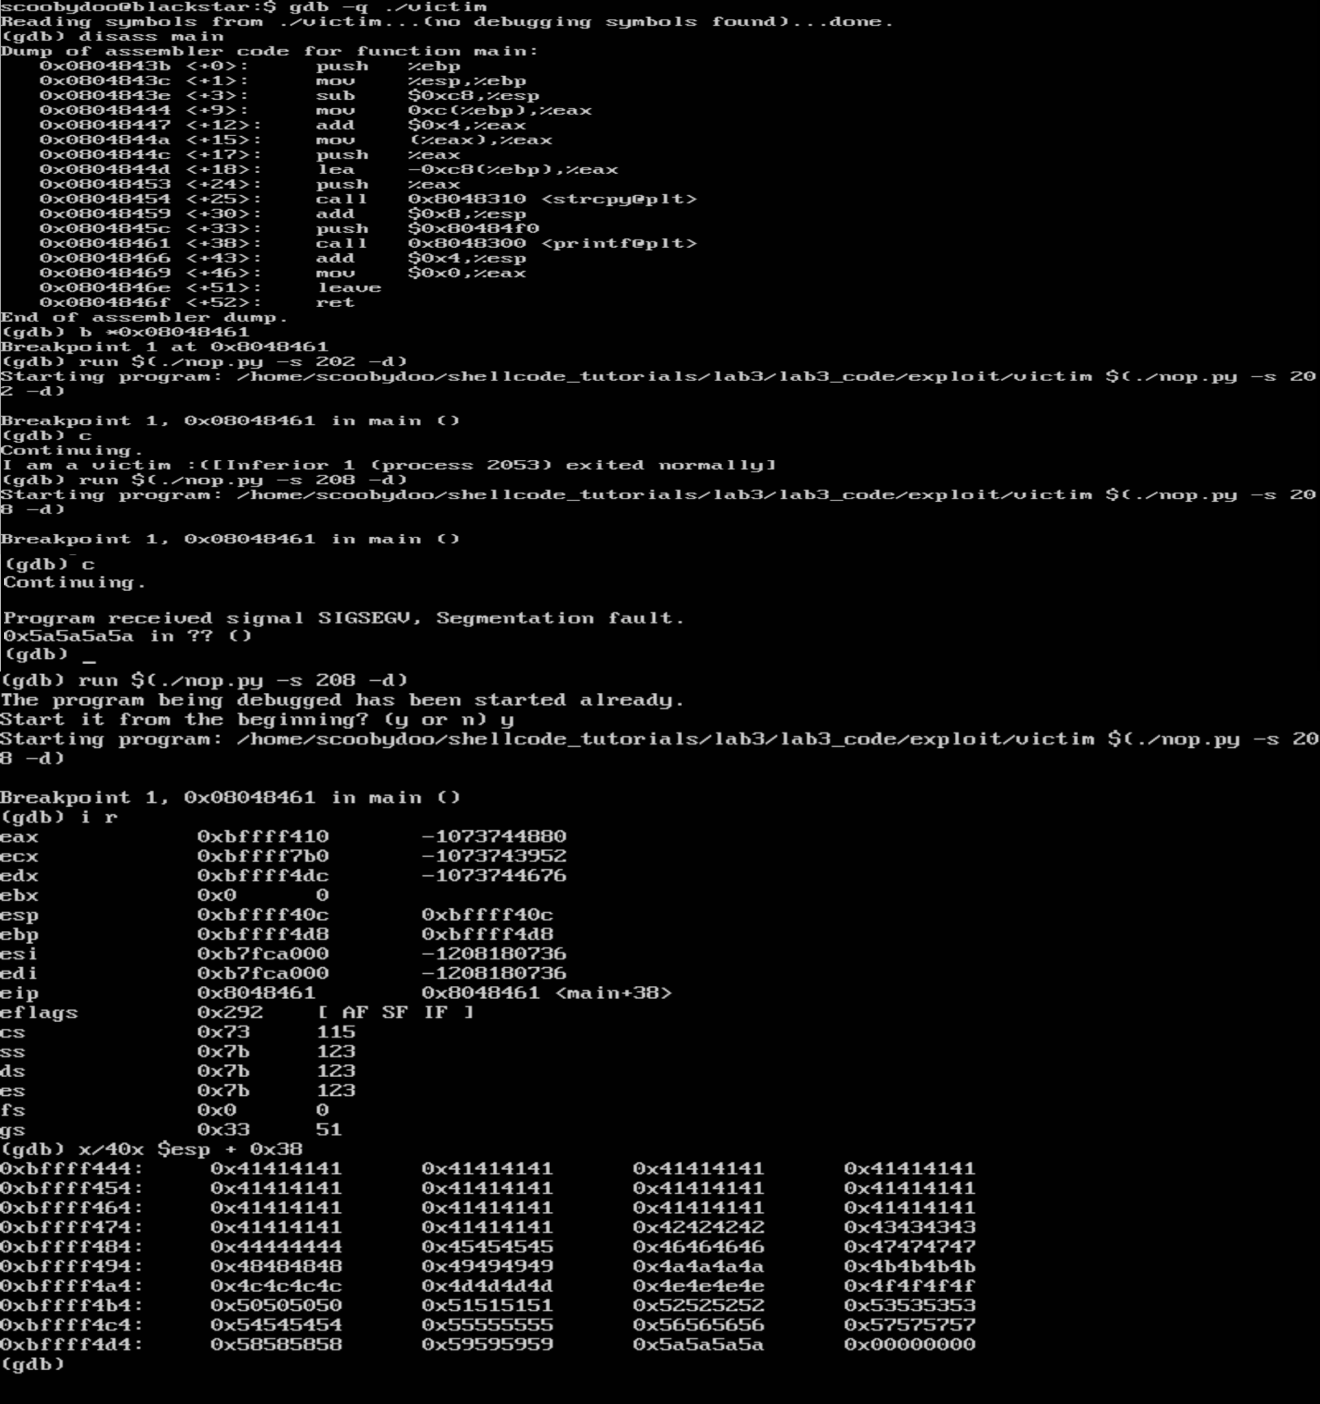
\includegraphics[width=16cm, height=16cm]{nop_gdb.png}
  \caption{Exploring victim.c with gdb}
\end{figure}
Next, let's store our shellcode in an environment variable using nop.py, shown in figure 8. This environment variable will contain a long string of x86 NOP instructions ('\textbackslash{x90}') followed by our shellcode at the end of the buffer.
\begin{figure}[H]
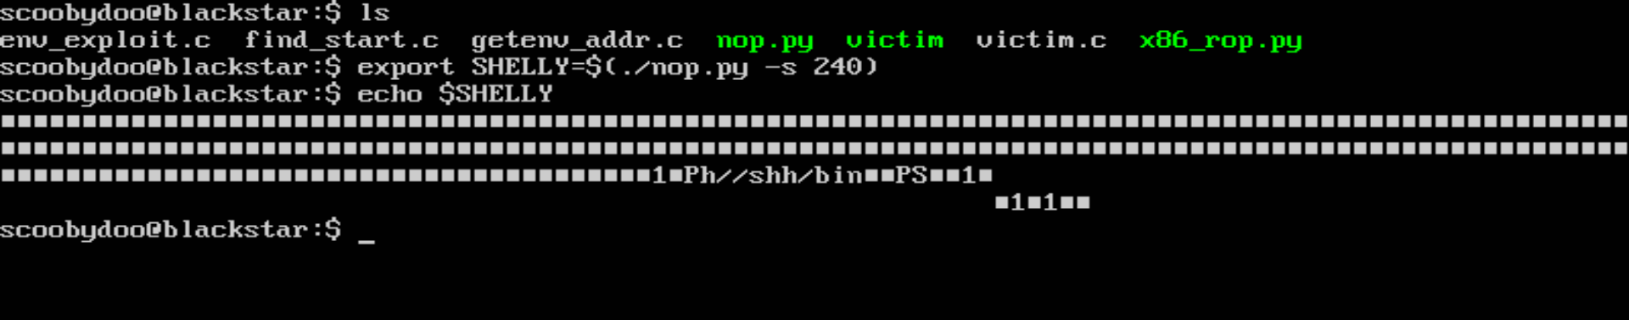
\includegraphics[width=16cm, height=4cm]{x86_nop_env.png}
  \caption{Exporting our shellcode as an environment variable using nop.py}
\end{figure}

Finally, we can create a buffer that is large enough to overflow victim.c that contains the address of our environment variable repeated over and over. We can then use this buffer as the argument to victim.c. This has been automated using the nop.py script, shown below. We create a buffer that is roughly of size 240, use the -e option to specify the name of our environment variable and the -t option to specify the target (used for calculating the address). This will output the buffer to stdout which we then use as an argument for victim.c. The buffer just repeats the same address over and over again so it will fill up the stack until it overflows into EIP, EIP will then be pointing to somewhere in our NOP sled, then slide down into our shellcode and give us a shell!

\begin{figure}[H]
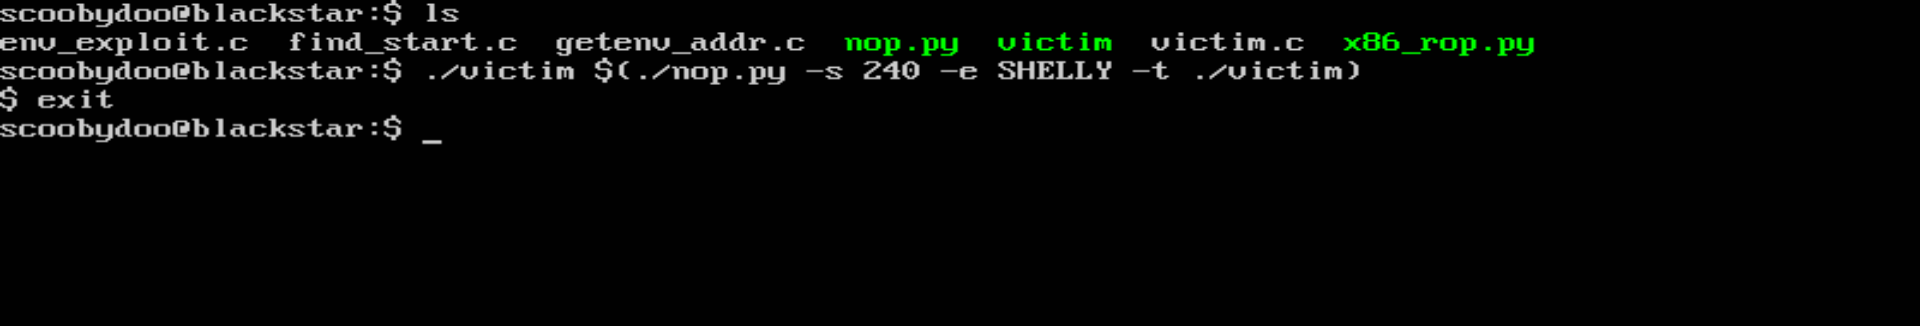
\includegraphics[width=16cm, height=3.5cm]{x86_nop_exploit.png}
  \caption{Overflowing victim.c with the address of our environment variable}
\end{figure}

A third method was created that uses the same idea of repeated environment variable addresses as shown above. This method was taken from pages 149-150 of the book \textit{Hacking: The Art of Exploitation} by Jon Erickson [11]. This gets rid of the need for a NOP sled by using a very accurate method to calculate the offset to the environment variable containing our shellcode. It will not be fully explained here but the code is contained in \textit{env\_exploit.c} and is fully commented.

\subsubsection{ARM}
In theory, we should be able to take the exact same steps as above (for x86) to exploit our target program. That is, store our shellcode (with a NOP sled) in an environment variable, then create a buffer with repetitions of the address of this environment variable, which can be passed into our victim program. Let's give it a try on different vulnerable program this time.\newline

This program is called \textit{overflow.c} and was taken from a paper by Aditya Gupta [12]. Below I will show me stepping through the program in GDB, first I will overflow the vulnerable buffer with the address of a function that doesn't normally get called in the program. Then I will try to do the same thing but pass the address of an environment variable containing our NOP sled and shellcode.

\begin{figure}[H]
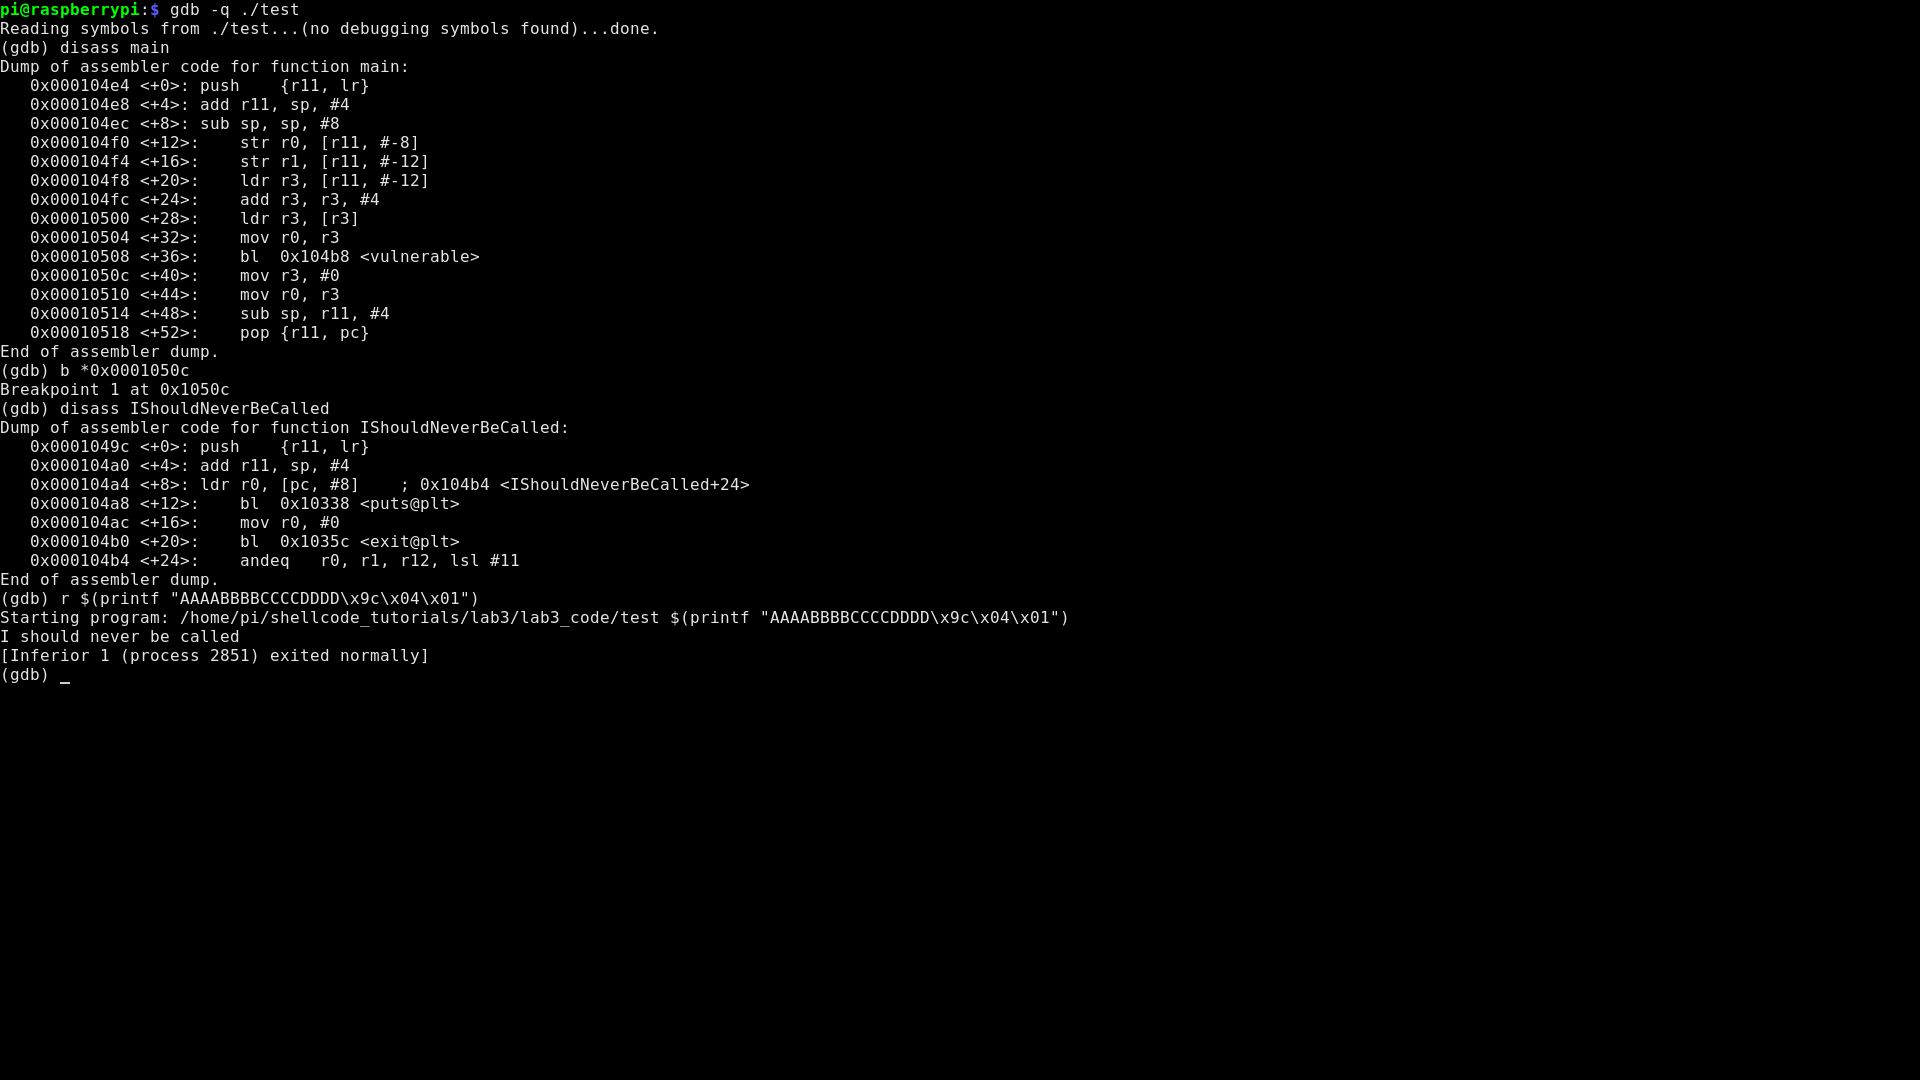
\includegraphics[width=16cm, height=10cm]{arm_overflow.png}
  \caption{Overflowing overflow.c with return address of the function IShouldNeverBeCalled}
\end{figure}

As you can see I put a break point after the function call that contains the vulnerable buffer, I then find the address of the function \textit{IShouldNeverBeCalled} and use printf to overflow the buffer, this calls the function and prints the message \textit{I should never be called}. An important note is in ARM we are trying to overflow the Link Register (LR) instead of EIP (x86), this is where the return address of a function is stored, it can also sometimes be stored in R0, more research is needed to know when each of these scenarios occur and if it matters. Since this worked let's try doing the same thing with a NOP sled stored in an environment variable.

\begin{figure}[H]
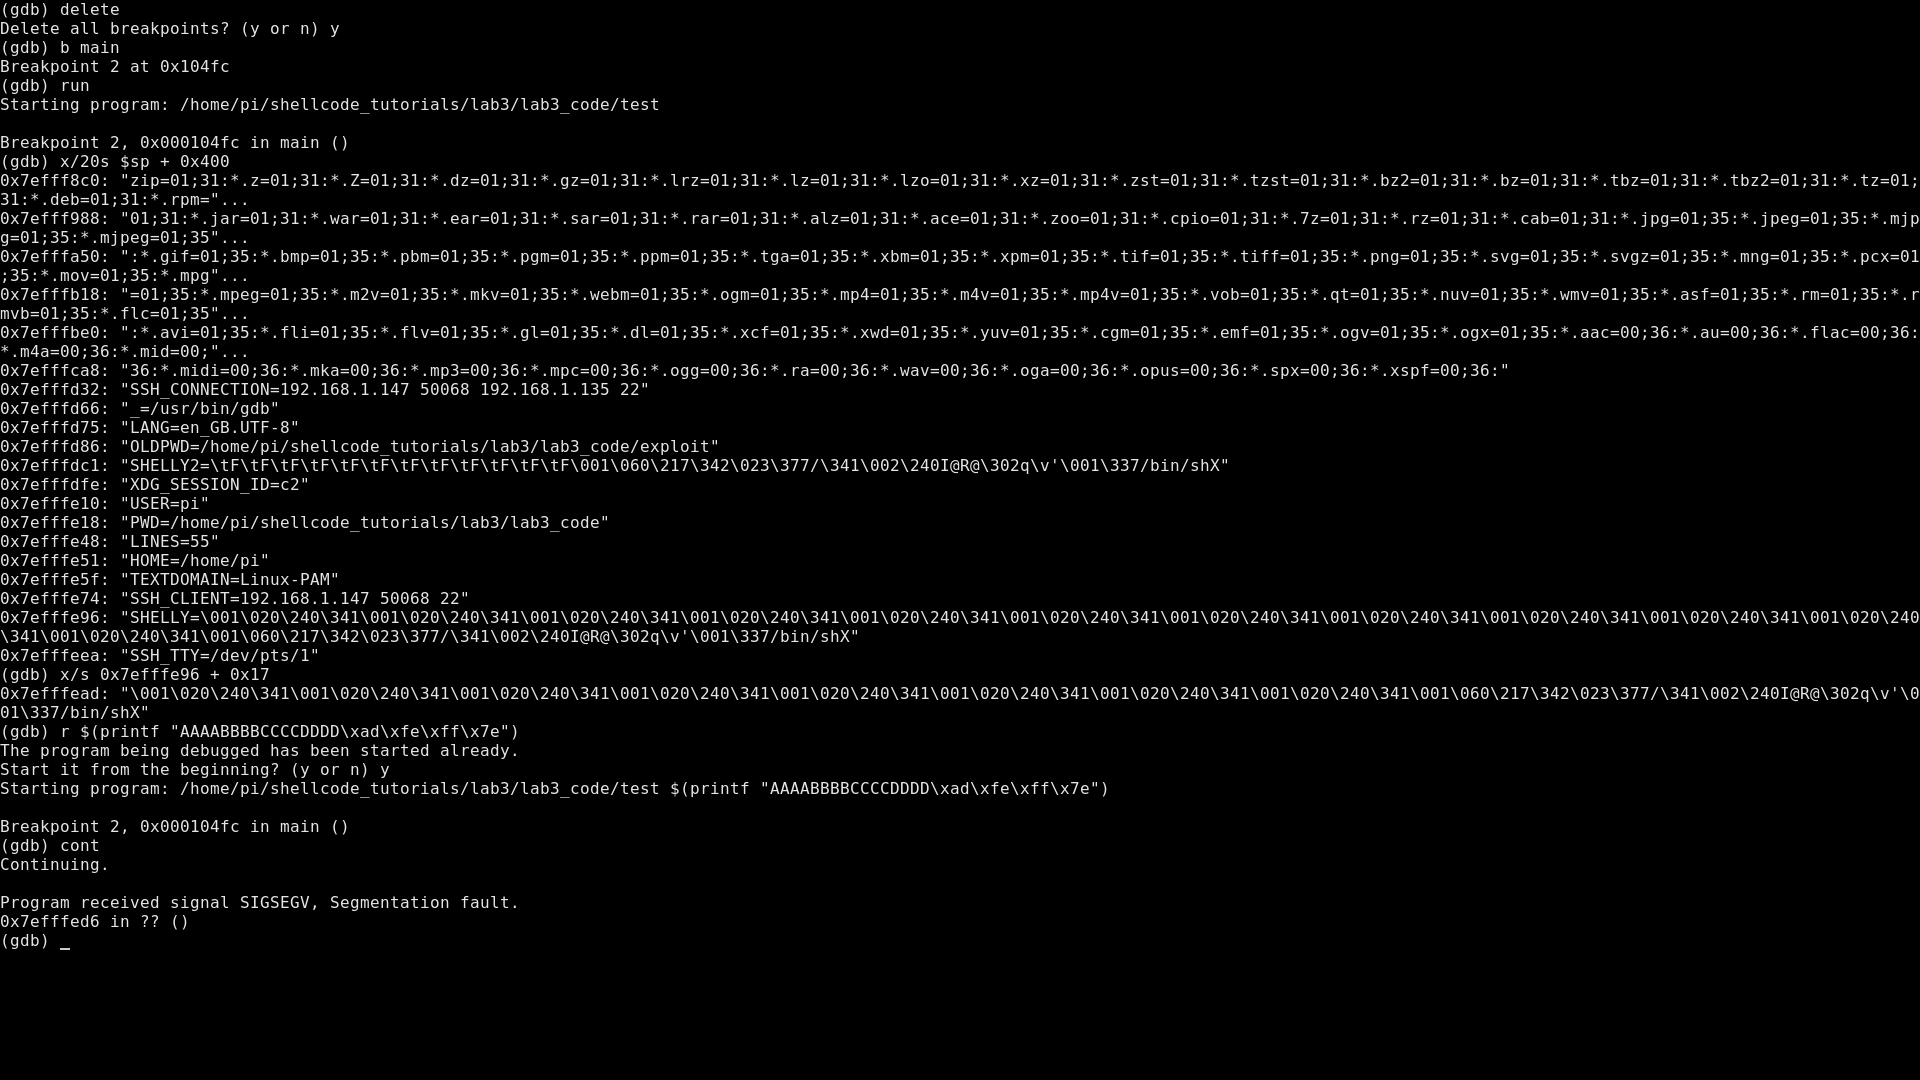
\includegraphics[width=16cm, height=10cm]{arm_overflow_nop.png}
  \caption{Overflowing overflow.c with return address of our NOP sled environment variable}
\end{figure}

This time around, a break point is set on main, the program is run, then we print the environment variables for our program by offsetting from the stack pointer (SP). We then use an address that is somewhere in the NOP sled contained in the SHELLY environment variable. We run the program with this address and.......no luck! What the willy wonka? Is our shellcode wrong? Is their alignment errors? Are we using a wrong instruction for our NOPs? Keep reading to find out!\newline

After further experimentation with the course instructor, we were finally able to determine the cause. It turns out that not only does our shellcode have to be four-byte aligned but the \textbf{address} of our environment variable must also be four-byte aligned (divisible by four). This makes sense, since the \textit{PC} increments by four bytes (except in THUMB mode). One other thing to note is that ARM NOP instructions are not a single opcode such as the ones on x86. This means we must not only have a four byte-aligned address, but the first instruction must be the first opcode of our ARM NOP instruction, not somewhere in the middle of it. To demonstrate this working, I added several NOP instructions to the top of good\_shell.s (MOV r1, r1), which will act as a NOP sled, after assembling the shellcode I then copied it into a raw binary which we can use to tinker around with our environment variable addresses.

\begin{figure}[H]
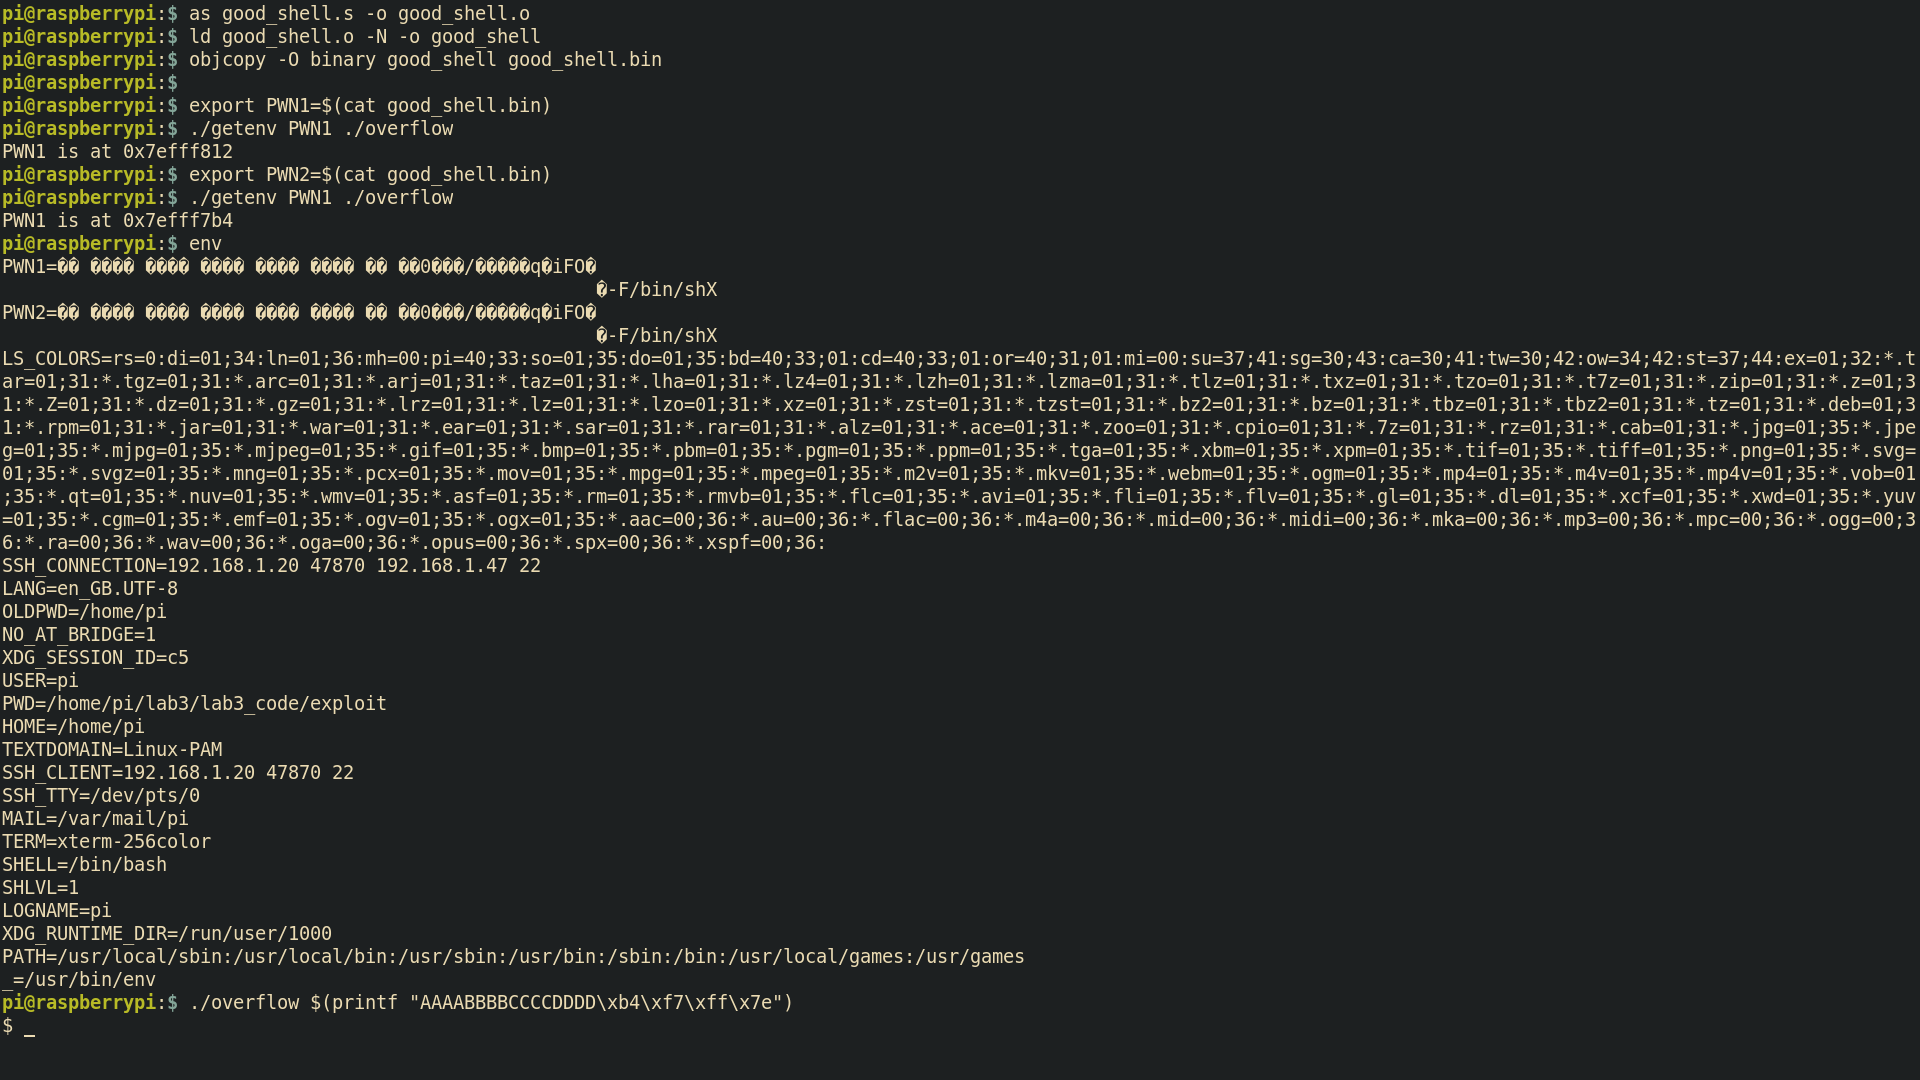
\includegraphics[width=16cm, height=10cm]{arm_overflow_nop_fixed.png}
  \caption{Overflowing overflow.c with byte-aligned NOP sled environment variable}
\end{figure}

First, I exported an environmental variable called \textit{PWN1}, then using the provided \textit{getenv} program I could see that the address was not divisible by 4. At this point you can try several things, such as making the name of your env variable longer, anything really, that allows you to manipulate the address of the variable until it is divisible by 4. I decided to try exporting another variable and see if I could use either one. In the example above, when I exported another variable it actually pushed my previous one up the stack (lower memory address) and coincidentally made it four-byte aligned. Finally, I overflowed the target programs stack with the address of this environment variable and successfully got a shell!

\subsection{ROP method}
ROP stands for Return Oriented Programming and is an exploitation method used to circumvent a non-executable stack. You'll notice when we compile of our program we use the "-z execstack" parameter, this makes the stack executable (our shellcode is executed on the stack). ROP is a general term, in Linux it is called ret2libc. When a program is compiled, it is linked with the libc Linux library, we can use GDB to find the memory locations of the functions located in the executable then overflow the instruction pointer with those addresses. This will make the instruction pointer return somewhere outside the stack into libc to execute the functions we tell it to.
\subsubsection{x86}
For x86 the technique involves having the function you want to call first, followed by the address you want to return to after the first function, then following that the arguments to pass to the first function. We can use the libc function system() with the argument "/bin/sh" then return to exit() (just to kill the target cleanly).
\begin{center}
  \begin{tabular}{ | l | c | r | }
    \hline
    FUNCTION ADDRESS & RETURN ADDRESS & ARGUMENTS \\ \hline
    system() & exit() & "    /bin/sh" \\ \hline
  \end{tabular}
\end{center}
A python script called x86\_rop.py has been written to automate the steps needed. Before running the script let's compile victim, this time omitting the "-z execstack" option then export an environment variable containing the argument for system().
\begin{verbatim}
gcc victim.c -fno-stack-protector -mpreferred-stack-boundary=2 -o victim
export SHELLY="     /bin/sh"
\end{verbatim}
\begin{figure}[H]
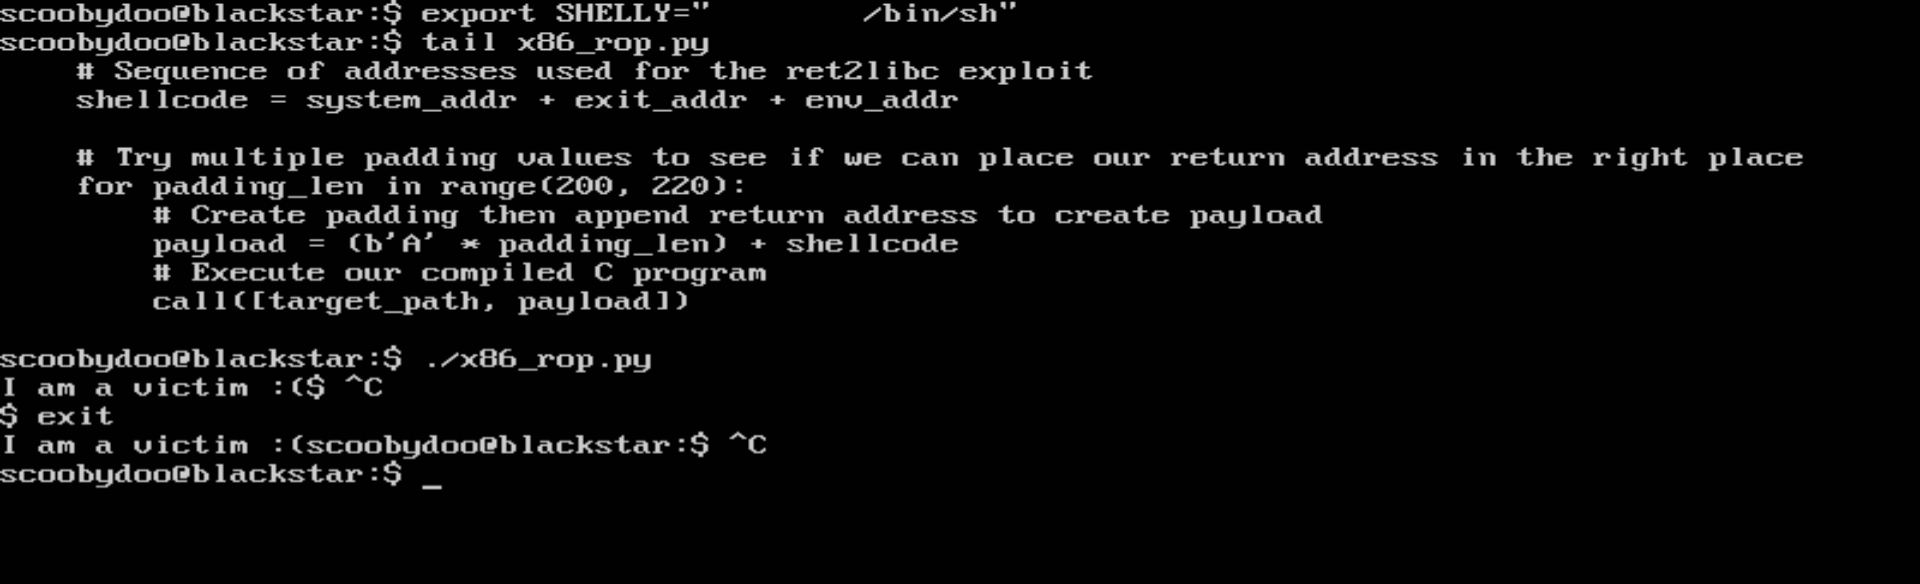
\includegraphics[width=16cm, height=4cm]{x86_rop_exploit.png}
  \caption{Overflowing victim.c with the ret2libc ROP addresses}
\end{figure}
The python script uses GDB to grab the addresses of system() and exit(), then uses ctypes to get the address of our environment variable. It then concatenates these three addresses together and bruteforces the buffer size needed to overflow EIP. The result is a shell, as shown above.


\subsubsection{ARM}
Here we are again at ARM exploitation, the ROP method for ARM is even harder to understand than our attempt at NOP on ARM. A serious amount of reading is needed to get ROP to work on ARM, this is because the way ARM accepts and returns arguments. In x86, arguments passed to functions are stored on the stack (this can be seen in the disassembly in Figure 7 above) this allows us to overflow the stack with the address of the functions we want to return to (system()) directly. As previously discussed, for ARM you must put your arguments in \textbf{registers} before a function is called, the function will then use these values then return through LR or R0. Thus in ARM we must create things called ROP gadgets which will have an instruction to put our return values into registers first which we can then use to overflow a buffer. That's wack, let's see an example of how this would work, this example is derived from slides by Andrea Sindoni [13].\newline

To start, let's think about the POP instruction, initially the POP instruction doesn't seem very useful, but if we look at what the POP instruction actually does, we see it just loads a value from the stack into a register. Example POP\{R0, R4, pc\} gets translated into:
\begin{verbatim}
ldr r0, [sp], #4
ldr r4, [sp], #4
ldr pc, [sp], #4
\end{verbatim}
This just loads a value from the stack into a register then increments the stack pointer. Great, so if we overflow a stack with a variable (say "/bin/sh"?) then put some garbage in for r4, and finally follow up with an address to a function call (say system()?), we can overflow the link register with this POP instruction followed by the needed addresses to call system("/bin/sh")!
\begin{center}
  \begin{tabular}{ | c | c | c | c | }
    \hline
    POP INSTRUCTION & R0 VALUE & R4 VALUE & FUNCTION ADDRESS \\ \hline
    POP\{R0, R4, pc\} & "/bin/sh" & "AAAA" & system() \\ \hline
  \end{tabular}
\end{center}
To find a POP instruction that does this, we can look in something most C programs always have. We know almost all C programs get linked during compilation with the libc library, this library contains a boat load of instructions, if we look in the right place we can find one that will use the POP instruction. Luckily Andrea [13] did this for us, let's take a peek at the address he points out in libc:
\begin{figure}[H]
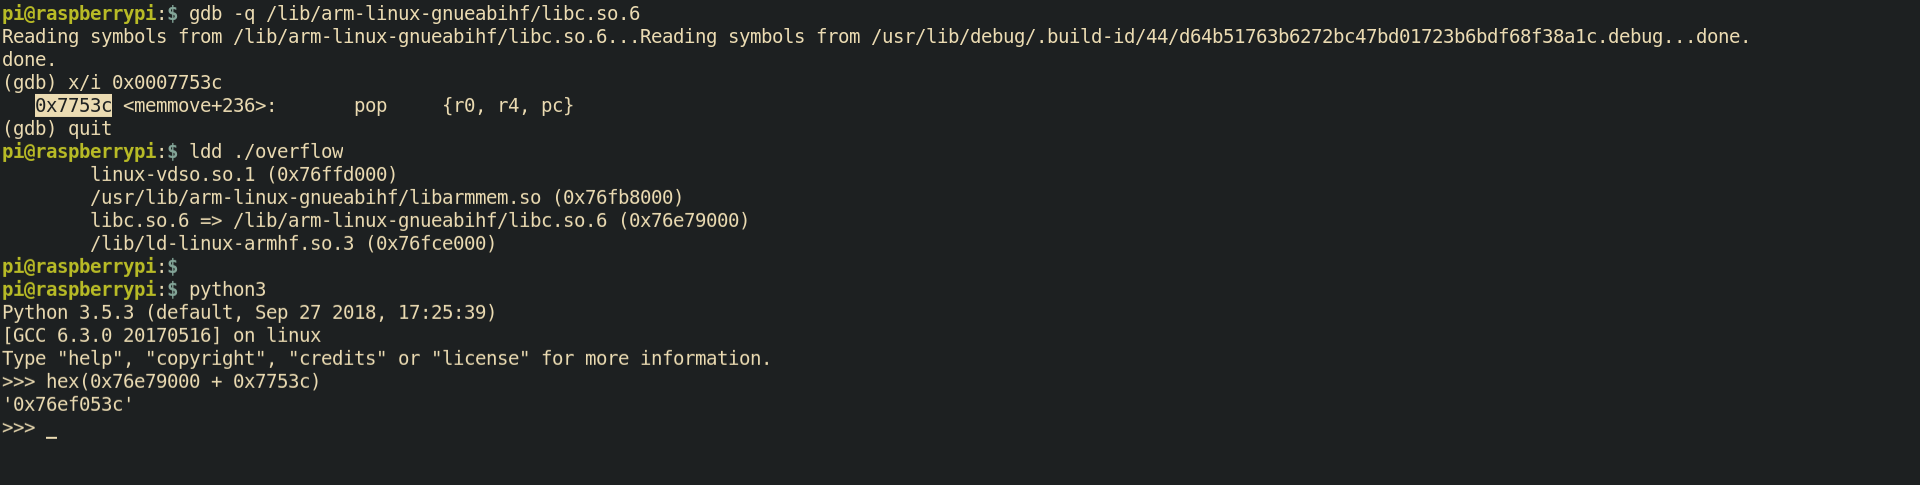
\includegraphics[width=16cm, height=4cm]{libc_pop.png}
  \caption{Well whaddya know?}
\end{figure}
According to the slides by Andrea [13] the address above will be offset by a default base address when libc is linked with an actual program, to find this we can simply run the \textit{ldd} command on our target executable and add the base address to the address found above (see figure above). OK then, let's get the address of "/bin/sh" by storing it in an environment variable, while we are at it let's get the address of system() by using gdb on our target program:
\begin{figure}[H]
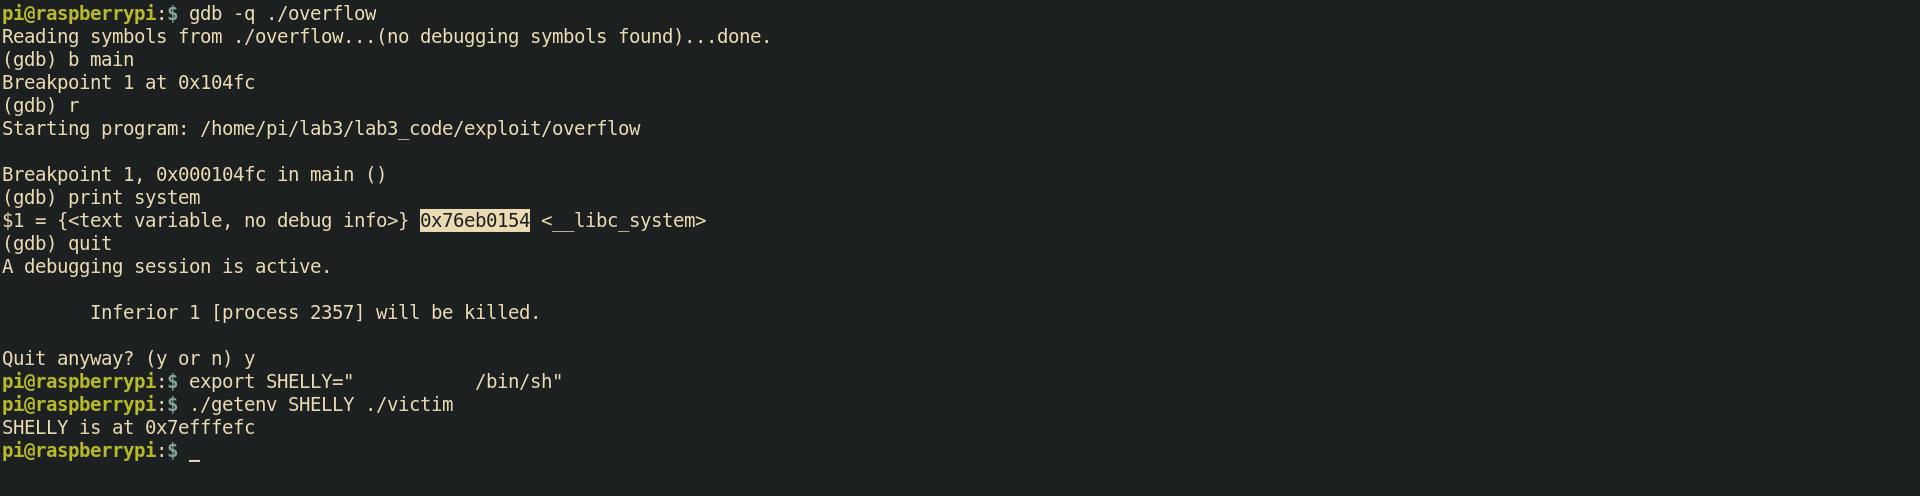
\includegraphics[width=16cm, height=4cm]{system_gdb.png}
  \caption{Getting address of "/bin/sh" and system() function}
\end{figure}
We now have all the things needed to create our buffer, it will look like this:
\begin{center}
  \begin{tabular}{| c | c | c | c | c | }
    \hline
    PADDING & POP INSTRUCTION & R0 VALUE & R4 VALUE & FUNCTION ADDRESS \\ \hline
    AAAAA... & "\textbackslash{x3c}\textbackslash{x05}\textbackslash{xef}\textbackslash{x76}" & "\textbackslash{xfc}\textbackslash{xfe}\textbackslash{xff}\textbackslash{x7e}" & "JUNK" & "\textbackslash{x54}\textbackslash{x01}\textbackslash{xeb}\textbackslash{x76}" \\ \hline
  \end{tabular}
\end{center}

\begin{figure}[H]
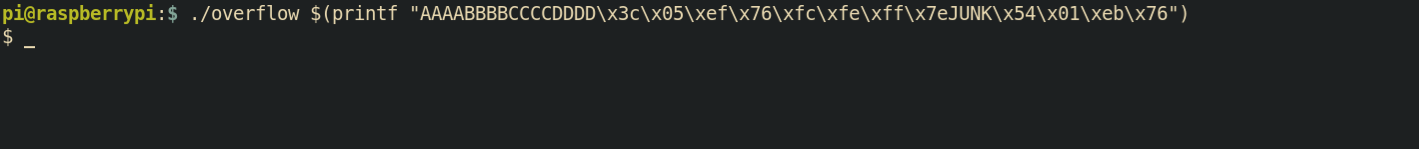
\includegraphics[width=16cm, height=2cm]{arm_rop.png}
  \caption{Overflowing overflow.c with the ret2libc ROP gadget}
\end{figure}

\section{Conclusions}
This lab highlighted the fundamentals of exploit development and common exploit techniques. This lab allowed us to learn an immense amount about how programs actually work especially at the assembly level. Buffers were pwned on x86  and ARM using both the NOP method and the more relevant and useful ROP method. Both taught and highlighted valuable information that can be expanded upon in the future.

\newpage

\section{References}

\begin{enumerate}
  \item\textbf{Python ctypes documentation}
    \newline\url{https://docs.python.org/3/library/ctypes.html}
  \item\textbf{StackOverflow: Python Ctype Segmentation Fault}
    \newline\url{https://stackoverflow.com/questions/19326409/python-ctype-segmentation-fault}
  \item\textbf{GNU libc function manuals}
    \newline\url{https://www.gnu.org/software/libc/manual/html\_node/Function-Index.html}
  \item\textbf{X86 Assembly/Interfacing with Linux}
    \newline\url{https://en.wikibooks.org/wiki/X86\_Assembly/Interfacing\_with\_Linux}
  \item\textbf{Linux Syscall Reference}
    \newline\url{https://syscalls.kernelgrok.com/}
  \item\textbf{Intel 64 and IA-32 Architecture Software Developer’s Manual}
    \newline\url{https://www.intel.com/content/dam/www/public/us/en/documents/manuals/64-ia-32-architectures-software-developer-instruction-set-reference-manual-325383.pdf}
  \item\textbf{Exploit Database: x86 execve shellcode}
    \newline\url{https://www.exploit-db.com/exploits/13375/}
  \item\textbf{Exploit Database: x86 exit shellcode}
    \newline\url{https://www.exploit-db.com/exploits/43688/}
  \item\textbf{Azeria Labs}
    \newline\url{https://azeria-labs.com/}
  \item\textbf{Exploit Database: ARM execve shellcode}
    \newline\url{https://www.exploit-db.com/exploits/45290/}
  \item\textbf{Hacking: The Art of Exploitation}
    \newline\url{https://en.wikipedia.org/wiki/Hacking:_The_Art_of_Exploitation}
  \item\textbf{A Short Guide on ARM Exploitation}
    \newline\url{https://www.exploit-db.com/docs/english/24493-a-short-guide-on-arm-exploitation.pdf}
  \item\textbf{ARM shellcode and exploit development by Andrea Sindoni}
    \newline\url{https://github.com/invictus1306/Workshop-BSidesMunich2018}
\end{enumerate}


\end{document}
